\subsubsection{Mediciones con imágenes}

El reconocimiento del entorno de desplazamiento del robot se puede realizar de muchas maneras, desde sensores ultrasónicos hasta cámaras fotográficas, y por supuesto dependiendo cual se selecciona la precisión de la medición va a aumentar o disminuir.
En base a los modelos anteriores del robot que utilizaron sensores de ultrasonido para determinar la distancia de los objetos que se encuentran en frente del robot, notamos que la precisión de los mismos no es suficiente. Es por ello que decidimos usar como alternativa una cámara fotográfica en conjunto con el procesamiento de imágenes para identificar los elementos que creamos necesarios dentro de la foto para determinar qué información podemos extraer de ahí, cómo interpretarla y finalmente influir en la estimación de la posición del robot. El beneficio que trae esta incorporación es poder aumentar la precisión de los movimientos que realiza el robot a través de una mejoría en la precisión de la estimación de la posición. \cite{dey2018hands}

Esta medición en tiempo real puede ser sumada como una entrada adicional al filtro de Kalman, pudiendo mejorar significativamente la estimación de la posición del robot. Esto es porque no teniendo ningún tipo de medición sobre el entorno y los movimientos, el único parámetro medible es la distancia recorrida por las ruedas y, como ya hemos visto en iteraciones anteriores, no es suficiente para determinar con precisión la ubicación del robot. En nuestro caso nos limitaremos solo a tomar mediciones de distancia desde el robot a los códigos QR, dejando el agregado de estas mediciones al Filtro de Kalman como futura implementación.

El microcontrolador ESP-32 cuenta con un modelo que incorpora la posibilidad de añadirle una cámara extraíble, desafortunadamente no es el mismo modelo el cual maneja la lógica del comportamiento del robot por lo cual fue necesario la incorporación de un nuevo microcontrolador y sumarle un sostén por encima del robot para que este sostenga la cámara y podamos obtener imágenes de manera más cómoda.

\begin{figure}[H]
   \centering
   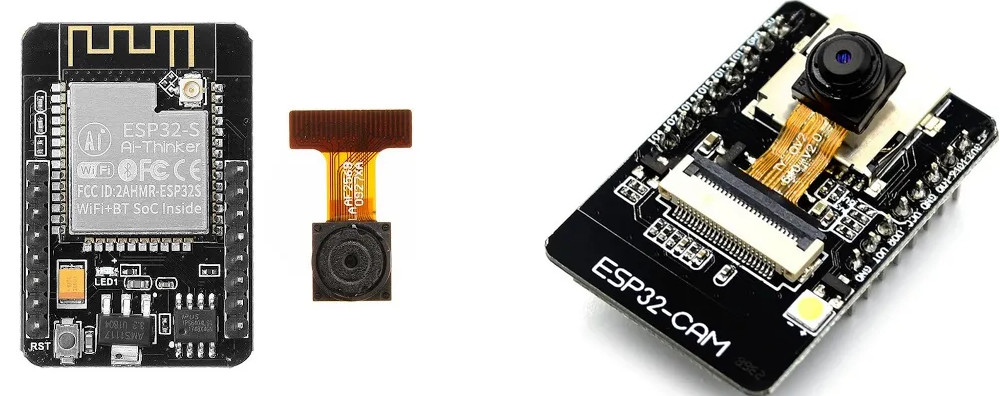
\includegraphics[width=0.6\linewidth]{images/esp32-cam.jpg}
   \caption{Microcontrolador ESP32-CAM con la cámara OV2640}
   \label{fig:esp32-cam}
\end{figure}

Con el solo hecho de tomar una fotografía con el microcontrolador, usamos la mayoría de su procesamiento en esa tarea. Realizando distintas pruebas con las resoluciones de imágenes que la cámara pone a disposición nos dimos cuenta que hasta es necesario añadirle un opción para habilitar una memoria RAM externa para almacenar las imágenes. Esto nos sirvió para darnos cuenta que no íbamos a poder realizar el procesamiento de las imágenes dentro del microcontrolador y lo mejor sería seguir acoplado al paradigma de IoT el cual nos plantea que este dispositivo solo va a servir para tomar la fotografía y enviarla a otro servidor el cual se va a encargar de procesar la imagen. En este caso, el procesamiento de las imágenes se hace en la PC host donde se tiene la interfaz de usuario ejecutándose, que recibe las imágenes por medio de MQTT.

\begin{figure}[H]
   \centering
   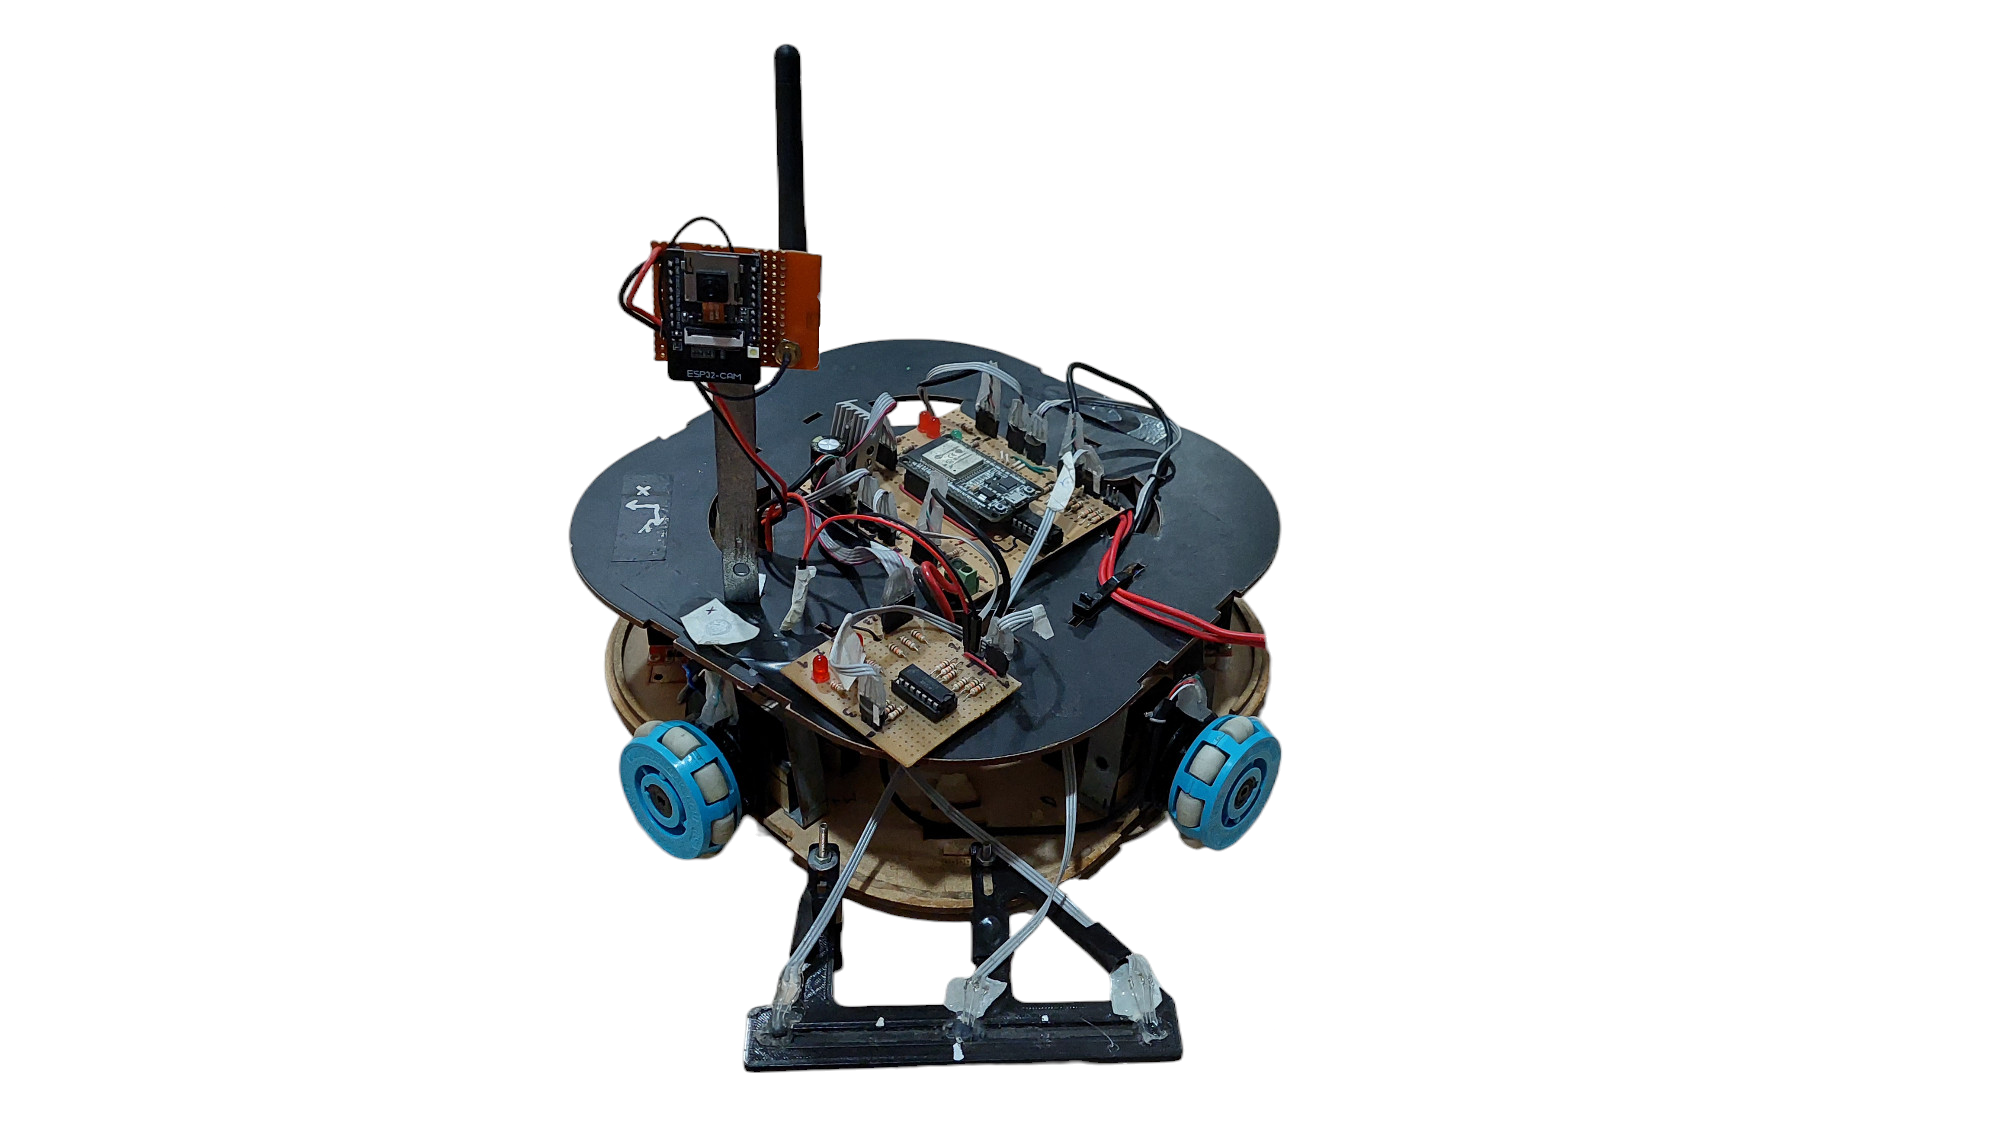
\includegraphics[width=1.0\linewidth]{images/robot_camara.png}
   \caption{Robot con la ESP32-CAM incorporada}
   \label{fig:robot_camara}
\end{figure}